\section{Assessment of the different approaches}

Based on our reference value from the section \ref{sec:reference}, we assess the performance of our two different approaches.

\subsection{Extension framework performance}

For our extension framework, we can say that it performs poorly.
For example, on Contiki with the RE-Mote board, the expected context switching time is $18.505\mu s$ but our framework measured a context switching time of $31.6162\mu s$.
With such a huge difference, we can not consider this approach as suited to build our benchmarking framework.

The reason behind this result is that the precision level of the real-time clock devices is not high enough.
During our experiments, we have measured that there is 32728 ticks per second with Contiki on the Z1 board.
In other words, a tick occurs every $30.5\mu s$.
This is why the minimal value measured on Contiki with the Z1 board is $30.5175\mu s$.

\subsection{Devices framework performance}

With the devices framework, we have better results than with our extension framework.
First, the measurements done with the framework differ only by 2.8\% with Contiki and 10.7\% with RIOT.
On Contiki, we have a maximum difference of $0.5\mu s$ with the reference value.
On RIOT, we have a maximum difference of $3\mu s$.
Moreover, we see with the figure \ref{fig:devices-comparison-contiki} that the distributions of the devices framework values match the distribution of the reference values on Contiki.
For RIOT, this issue is discussed in the next section.
Therefore, we can considerate this approach suited for our benchmarking framework.

\begin{figure}[!ht]
  \centering
  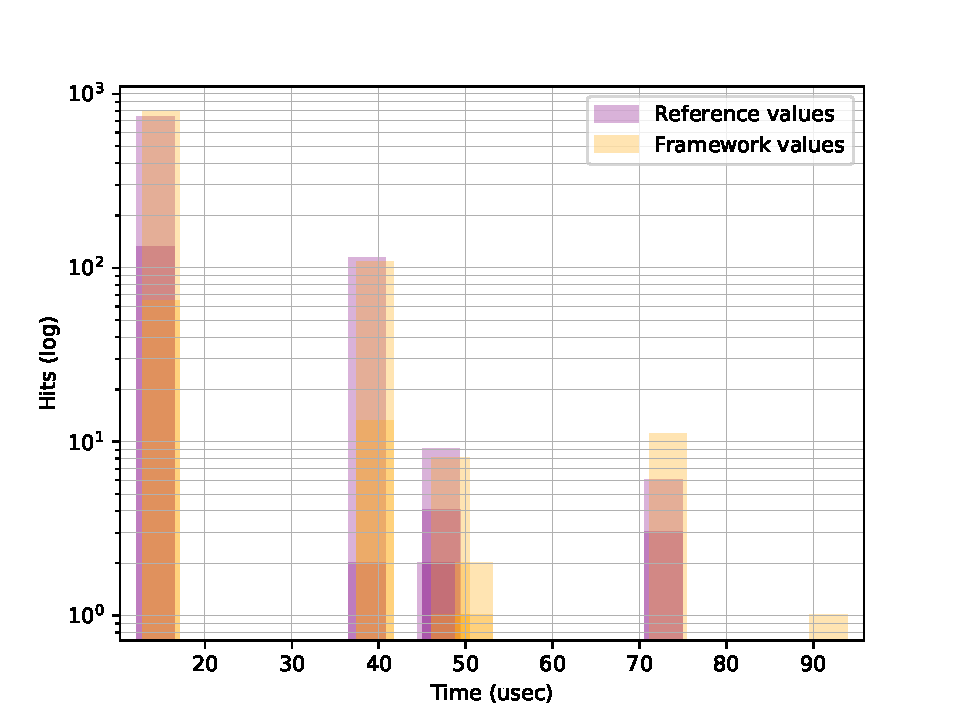
\includegraphics[scale=.7]{assets/comparison-devices-framework-contiki-remote.pdf}
  \caption*{Measurements made on the RE-Mote board}
% \end{figure}

% \begin{figure}[!ht]
  \centering
  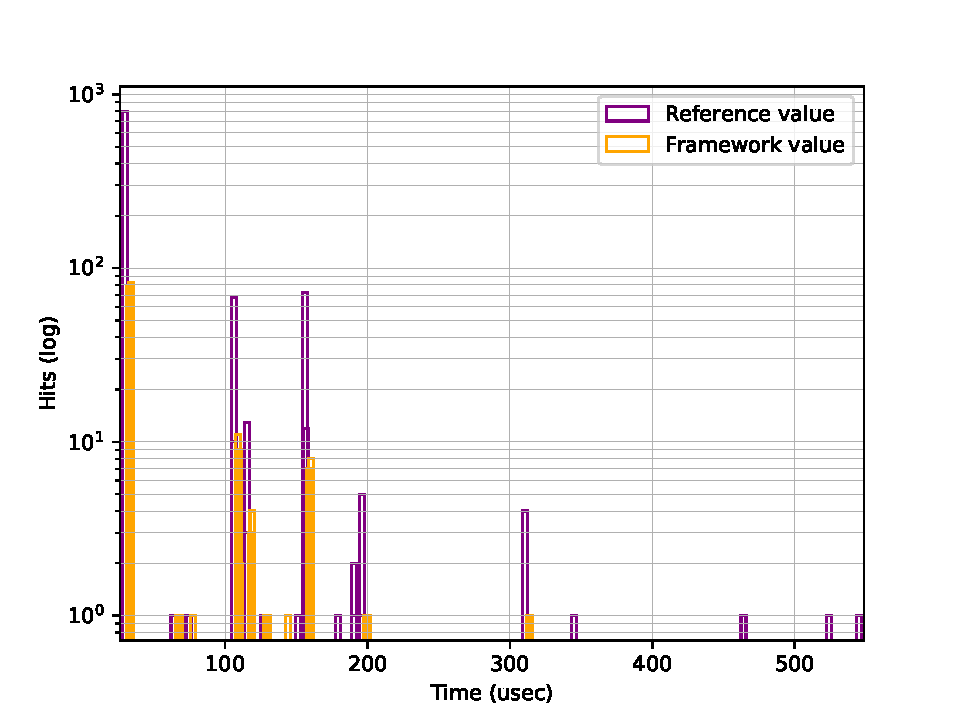
\includegraphics[scale=.7]{assets/comparison-devices-framework-contiki-z1.pdf}
  \caption*{Measurements made on the Z1 board}
  \caption{Comparison of the devices framework with the reference value on Contiki\label{fig:devices-comparison-contiki}}
\end{figure}